\subsection*{a} 

\vspace{10pt}
\emph{Parity} \\
\vspace{10pt} \\
Let us consider a wavefunction $\psi(\ve r)$. One can define the parity operator $\hat P$ as an operator such that 
\begin{equation*}
    \hat P \, \psi(\ve r) = \psi(-\ve r)
\end{equation*}
Since
\begin{equation}
    \hat P^2 \, \psi(\ve r) = \hat P \, \psi(-\ve r) = \psi(\ve r)
    \label{eq:eigenvalue_equation_parity}
\end{equation}
the eigenvalues of the parity operator are $\pm 1$ and the corresponding eigenfunctions are the odd (eigenvalue $-1$) and even (eigenvalue $+1$) wavefunctions. If the wavefunction
describes the state of particle, and the state is an eigenstate of the parity operator, the corresponding eigenvalue is also said to be the (intrinsic) parity of the particle. Formally
\begin{equation*}
    \hat P \psi(\ve r) = \pi \psi(\ve r)
\end{equation*}
and $\pi$ is the (intrinsic) parity of the particle. \\
Let us consider a system of two particles $A+B$ described by a wavefunction $\psi_{AB}(\ve{r}_A, \ve{r}_B)$. It can be proven that the parity of the system is given by 
\begin{equation*}
    \hat P |psi_{AB} = \pi_A \pi_B (-1)^l \psi_{AB}
\end{equation*}
where $l$ denotes the orbital angular momentum quantum number of the relative motion. Hence in a reaction of the type $A+B \rightarrow C+D$ described by a hamiltonian $\hat H$ that commutes with parity,
parity is conserved or, in other words
\begin{equation*}
    \pi_A \pi_B (-1)^{l_{AB}} = \pi_C \pi_D (-1)^{l_{CD}} 
\end{equation*}
This, for example, is not the case of the weak interaction where, in general, the hamiltonian operator does not commute with the parity operator. \\
\vspace{10pt} \\

\raggedright\emph{Charge conjugation} \\
\vspace{10pt} 
The charge conjugation operator is an operator that changes the sign of all the forces' quantum charges, specifically electric charge, baryon number, lepton number, flavor charges, isosping, \dots In particular, if applied to a particle, the C-parity operator 
transforms the particle into its antiparticle. If a particle is in a state $\left| \psi \right\rangle$ then the action of the conjugation operator reads 
\begin{equation*}
    \hat C \, \left| \psi \right\rangle = \left| \bar\psi \right\rangle
\end{equation*}
where $\left| \bar\psi \right\rangle$ represents the antiparticle's state. \\
The eigenstates of the C-parity operator are the systems neutral to all force charges like the photon or particle-antparticle bound states. In this case
\begin{equation*}
    \hat C \, \left| \psi \right\rangle = C_{\psi} \left| \psi \right\rangle
\end{equation*}
and $C_{\psi}$ is said to be the C-parity of the particle. As for the the parity operator, the eigenvalues can be only $\pm 1$. \\
Both P-parity and C-parity are conserved in the processes governed by all the fundamental forces \href{https://en.wikipedia.org/wiki/Weak_interaction#Violation_of_symmetry}{but the weak force}.

\subsection*{b}
The notation $^3S_1$ stands for $L=1$ $S=1$ and $J=1$. The $J/\Psi$ Meson is a bound state of a charm quark and an anti-charm quark. By applying the C-parity operator on the state $\left|J/\Psi\right\rangle$ and noting that each quark is transformed into the other one,
one obtains that the C-parity of the $J/\psi$ meson is -1 (the only contribution is due to the angular momentum).
\begin{equation*}
    \hat C \left|J/\Psi\right\rangle = (-1)^J\left|J/\Psi\right\rangle = -\left|J/\Psi\right\rangle
\end{equation*}
\subsection*{c}
$^{15}$N atom has 7 protons and 8 neutrons. Since the neutrons (in the ground state) are all coupled (each sub-shell admits two nucleons) they do not contribute to  the spin of the nucleus and the parity contribution is $+1$. Instead the protons configuration
of the $^{15}$N atom in the ground state is $(1s)^2 \, (1p_{3/2})^2 \, (1p_{1/2})^1$: only the last proton contributes to the interested quantities. Since the orbital $p$ represents the quantum number $l=1$ the parity of the the nucleus is the product of the neutrons 
an protons contribution, that is $(+1) \cdot (-1)^1 = -1$. The spin is then $1/2$. \\
There are three possible alternatives for the first excited state, all of which consists in moving a proton or a neutron to another level starting from the ground state configuration.
\begin{enumerate}
    \item Move the $1p_{1/2}$ proton to the $1d_{5/2}$ level \\ $\quad \longrightarrow \quad$ the new proton configuration is $(1s)^2 \, (1p_{3/2})^2 \, (1p_{1/2})^{-2} \, (1d_{5/2})^1$ and the spin-parity is $5/2^+$.
    \item Move the $1p_{3/2}$ proton to the $1p_{1/2}$ level \\ $\quad \longrightarrow \quad$ the new proton configuration is $(1s)^2 \, (1p_{3/2})^{-1} \, (1p_{1/2})^2$ and the spin-parity is $3/2^-$.
    \item Move the $1p_{1/2}$ neutron to the $1d_{5/2}$ level \\ $\quad \longrightarrow \quad $ the new neutorn configuration is $(1s)^2 \, (1p_{3/2})^2 \, (1p_{1/2})^{-1} \, (1d_{5/2})^1$. The parity here is non-trivial because of the angular momemnta addition rules.
\end{enumerate}
By looking at the suggested table, one can notice that the first excited state is described by configuration $1$, the second excited state by configuration $3$ and the third excited state is described by configuration $2$.


\begin{figure}
    \centering
    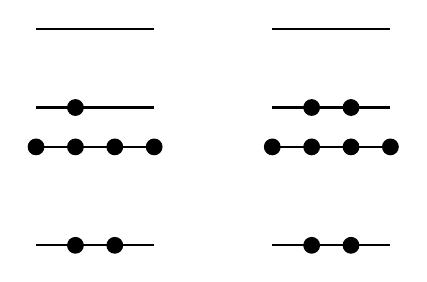
\begin{tikzpicture}
        
        % Protons
        \foreach \x in {0, 3}{
            \foreach \y in {0, 1.25, 1.75, 2.75}{
                \draw [thick] (\x, \y) -- ++(1.5, 0);
            }
            \node[draw, circle, inner sep=2pt, fill] at (\x+0.5, 0){};
            \node[draw, circle, inner sep=2pt, fill] at (\x+1, 0)(1.5,0){};
            \node[draw, circle, inner sep=2pt, fill] at (\x, 1.25){};
            \node[draw, circle, inner sep=2pt, fill] at (\x+0.5, 1.25){};
            \node[draw, circle, inner sep=2pt, fill] at (\x+1.5, 1.25){};
            \node[draw, circle, inner sep=2pt, fill] at (\x+1, 1.25){};
            \node[draw, circle, inner sep=2pt, fill] at (\x+0.5, 1.75){};
        }
        \node[draw, circle, inner sep=2pt, fill] at (4, 1.75){};
    \end{tikzpicture}
    \caption{nothing}
    \label{fig:nitrogen_nucleons_ground_state}
\end{figure}


\begin{figure}
    \centering
    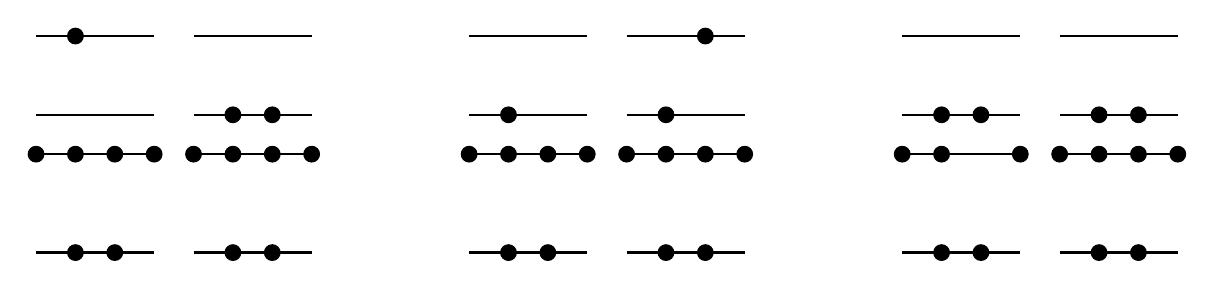
\begin{tikzpicture}

        % Protons
        \foreach \x in {0.5, 6, 11.5}{
            \foreach \y in {0, 1.25, 1.75, 2.75}{
                \draw [thick] (\x, \y) -- ++(1.5, 0);
            }
            \node[draw, circle, inner sep=2pt, fill] at (\x+0.5, 0){};
            \node[draw, circle, inner sep=2pt, fill] at (\x+1, 0)(1.5,0){};
            \node[draw, circle, inner sep=2pt, fill] at (\x, 1.25){};
            \node[draw, circle, inner sep=2pt, fill] at (\x+0.5, 1.25){};
            \node[draw, circle, inner sep=2pt, fill] at (\x+1.5, 1.25){};
        }
        
        % 1p 1/2 proton
        \node[draw, circle, inner sep=2pt, fill] at (1, 2.75){};
        \node[draw, circle, inner sep=2pt, fill] at (6.5, 1.75){};
        \node[draw, circle, inner sep=2pt, fill] at (12, 1.75){};

        % 1p 1/2 neutron
        \node[draw, circle, inner sep=2pt, fill] at (3.5, 1.75){};
        \node[draw, circle, inner sep=2pt, fill] at (9, 2.75){};
        \node[draw, circle, inner sep=2pt, fill] at (14.5, 1.75){};

        % 1p 3/2 proton
        \node[draw, circle, inner sep=2pt, fill] at (1.5, 1.25){};
        \node[draw, circle, inner sep=2pt, fill] at (7, 1.25){};
        \node[draw, circle, inner sep=2pt, fill] at (12.5, 1.75){};

        % Neutrons
        \foreach \x in {2.5, 8, 13.5}{
            \foreach \y in {0, 1.25, 1.75, 2.75}{
                \draw [thick] (\x, \y) -- ++(1.5, 0);
            }
            \node[draw, circle, inner sep=2pt, fill] at (\x+0.5, 0){};
            \node[draw, circle, inner sep=2pt, fill] at (\x+1, 0)(1.5,0){};
            \node[draw, circle, inner sep=2pt, fill] at (\x, 1.25){};
            \node[draw, circle, inner sep=2pt, fill] at (\x+0.5, 1.25){};
            \node[draw, circle, inner sep=2pt, fill] at (\x+1, 1.25){};
            \node[draw, circle, inner sep=2pt, fill] at (\x+1.5, 1.25){};
            \node[draw, circle, inner sep=2pt, fill] at (\x+0.5, 1.75){};
        }

    \end{tikzpicture}
    \caption{nothing}
    \label{fig:nitrogen_nucleons_excited_states}
\end{figure}

\subsection*{d}
The third excited state is the one that has $J^p = \frac{3}{2}^-$. From this state the nucleus can decay into the second excited state, the first excited state and the ground state. 
Let us first consider the decay to the ground state. When the excited proton returns to the $1p_{3/2}$ level there is no change in parity 
and one has that $\Delta J = J_{exc} - J_{ground} = 1$. This means that one must have odd-L magnetic fields and even-L electric fields. \\
Because of the general selection rules in the gamma decays one has that, said $L$ the photon's angular momentum
\begin{gather*}
    |J_{exc} - J_{ground}| \leq L \leq J_{exc} + J_{ground} \qquad \longrightarrow \qquad 1 \leq L \leq 2
\end{gather*}
The allowed states are
\begin{equation*}
    M_1, E_2
\end{equation*}
For $A=15$ one has that (ADD REFERENCE TO KRANE)
\begin{equation}
    \frac{\lambda(E_2)}{\lambda(M_1)} \approx 10^{-3}
\end{equation}
hence we expect the $M_1$ decay to be the most probable one, but with a non-neglectable contribution of $E_2$. \\
In an analogous way one can find that for the decays to the second and first excited states the relations reported in table \ref{tab:gamma_transitions}.
\begin{table}[htbp]
    \centering
    \begin{tabular}{cccccc}
        \toprule
        Transition & $\Delta E$ & $\Delta \pi$ & $L$ & Fields & Dominants\\
        \midrule
        $3 \to 0$ & $\approx 6.3~MeV$ & no & $1 \leq L \leq 2$ & $M_1, E_2$ & $M_1, E_2$ \\
        $3 \to 1$ & $\approx 1~MeV$ & yes & $1 \leq L \leq 4$ & $E_1, M_2, E_3, M_4$ & $E_1$\\
        $3 \to 2$ & $\approx 1~MeV$ & yes & $1 \leq L \leq 2$ & $E_1, M_2$ & $E_1$ \\
        \bottomrule
    \end{tabular}
    \caption{}
    \label{tab:gamma_transitions}
\end{table}
For the transition $2 \to 1$ one has that the dominant field is $E_2$ ($2 \leq L \leq 3$ and no parity change) while for the decay 
$2 \to 0$ the dominant field is $E_1$ ($0 \leq L \leq 1$ and parity change). Hence from the second excited state the nucleus cand ecay to the ground state 
via $E_1$ radiation, or it can decay to the first excited state via $E_2$ radiation. By comparing probabilities (REFERENCE TO KRANE)
\begin{equation*}
    \frac{P_{2 \to 0}}{P_{2 \to 1}} \approx \frac{\lambda(E_1)}{\lambda(E_2)} = \frac{1}{7.3} \cdot 10^{7} \cdot  A^{-2/3} > 1
\end{equation*}